\documentclass[12pt,a4paper]{article}

% --- Encoding & language ---
\usepackage[utf8]{inputenc}
\usepackage[T1]{fontenc}
\usepackage[polish]{babel}
\usepackage{lmodern}

% --- Math & symbols ---
\usepackage{amsmath,amssymb,amsthm}
\usepackage{mathtools}
\usepackage{bm}

% --- Layout ---
\usepackage[margin=2.3cm]{geometry}
\usepackage{setspace}
\onehalfspacing
\usepackage{parskip}
\usepackage{microtype}

% --- Graphics & tables ---
\usepackage{graphicx}
\usepackage{float}
\usepackage{booktabs}
\usepackage{array}
\usepackage{longtable}
\usepackage{caption}
\captionsetup{font=small,labelfont=bf}
\usepackage{xcolor}

% --- Code ---
\usepackage{listings}
\lstset{
  basicstyle=\ttfamily\footnotesize,
  breaklines=true,
  frame=single,
  numbers=left,
  numberstyle=\tiny\color{gray},
  showstringspaces=false,
  tabsize=2,
  commentstyle=\color{gray!70!black},
  keywordstyle=\color{blue!60!black}\bfseries,
  stringstyle=\color{green!50!black},
  language=Python
}

% --- Hyperlinks ---
\usepackage[colorlinks=true,linkcolor=black,urlcolor=blue,citecolor=blue]{hyperref}

% --- Header / footer ---
\usepackage{fancyhdr}
\setlength{\headheight}{14.5pt}
\addtolength{\topmargin}{-2.5pt}
\pagestyle{fancy}
\fancyhf{}
\fancyhead[L]{\small \textit{XAI: Permutation Importance, PDP/ICE, SHAP, LIME}}
\fancyfoot[C]{\thepage}
\renewcommand{\headrulewidth}{0.4pt}

% --- Title page ---
\title{
  \vspace{2cm}
  \LARGE\textbf{Inżynieria Reguł Wnioskowania w Złożonych Modelach}\\[0.6cm]
  \Large Laboratorium 5\\[0.4cm]
  \large \textit{XAI: Permutation Importance, PDP/ICE, SHAP, LIME}\\[0.3cm]
  \normalsize Wariant: \textbf{0/1 (brak wariantu 8 — zadanie jednolite)}
}
\author{Jakub Jurzak 59099}
\date{07.05.2026}

\begin{document}
\maketitle
\thispagestyle{empty}
\newpage

\tableofcontents
\newpage

\section{Cel zadania}
Praktyczne zastosowanie metod interpretowalności modeli ML w domenie medycznej. Porównanie globalnych (PI, PDP, SHAP summary) i lokalnych (ICE, SHAP waterfall, LIME) wyjaśnień decyzji klasyfikatora przeżycia.

\section{Opis problemu}
Modele ensemblowe (Random Forest) są nieliniowe i nieintuicyjne. W praktyce klinicznej wymagana jest możliwość uzasadnienia każdej predykcji (rozporządzenie AI Act, dobre praktyki kliniczne). Stąd potrzeba narzędzi XAI.

\section{Opis danych}
Zbiór z lab1: \texttt{prostate\_cancer\_synth.csv} ($N=600$). Cechy: \texttt{age, psa, gleason\_score, comorbidities}, OHE dla \texttt{tumor\_stage}, \texttt{treatment}. Etykieta: \texttt{survived}.

\section{Opis metod}
\textbf{Model:} \texttt{RandomForestClassifier} (300 drzew, \texttt{class\_weight=balanced}). \\\textbf{PI:} \texttt{permutation\_importance} z metryką ROC AUC ($n\_repeats=20$).\\\textbf{PDP/ICE:} \texttt{PartialDependenceDisplay} dla cech \texttt{age}, \texttt{psa}, \texttt{gleason\_score} (PDP) oraz krzywych ICE dla \texttt{age} i \texttt{psa}.\\\textbf{SHAP:} \texttt{TreeExplainer}, \texttt{summary\_plot} (globalnie) oraz \texttt{waterfall} dla pacjenta \#0.\\\textbf{LIME:} \texttt{LimeTabularExplainer} z dyskretyzacją cech ciągłych, 8 cech w wyjaśnieniu.

\section{Opis implementacji}
Plik \texttt{lab5/lab5\_solution.py}. Struktura: \texttt{prepare\_features} $\to$ trening RF $\to$ \texttt{permutation\_importance} $\to$ \texttt{plot\_pdp/plot\_ice} $\to$ \texttt{shap\_summary/shap\_waterfall} $\to$ \texttt{lime\_explain}.

\section{Obliczenia}
Wskaźniki bazowe modelu: \textbf{accuracy} = 0.867, \textbf{ROC AUC} = 0.784.

\begin{table}[H]
\centering
\begin{tabular}{lrr}
\toprule
feature & importance & std \\
\midrule
gleason\_score & 0.1260 & 0.0380 \\
age & 0.0666 & 0.0281 \\
comorbidities & 0.0598 & 0.0226 \\
tumor\_stage\_T3 & 0.0513 & 0.0152 \\
psa & 0.0451 & 0.0263 \\
treatment\_surgery & 0.0334 & 0.0240 \\
treatment\_radiation & 0.0136 & 0.0110 \\
tumor\_stage\_T4 & 0.0125 & 0.0093 \\
treatment\_watch & 0.0111 & 0.0102 \\
tumor\_stage\_T2 & -0.0015 & 0.0147 \\
\bottomrule
\end{tabular}

\caption{Permutation Importance --- ranking cech.}
\label{tab:pi}
\end{table}

Wyjaśnienie LIME dla pacjenta \#0:

\begin{table}[H]
\centering
\begin{tabular}{lr}
\toprule
warunek na cesze & wkład LIME \\
\midrule
gleason\_score <= 7.00 & 0.0994 \\
tumor\_stage\_T4 <= 0.00 & 0.0923 \\
treatment\_watch <= 0.00 & 0.0666 \\
age <= 62.00 & 0.0463 \\
tumor\_stage\_T3 > 0.00 & -0.0371 \\
treatment\_surgery <= 0.00 & -0.0259 \\
psa <= 4.70 & 0.0250 \\
0.00 < comorbidities <= 1.00 & -0.0124 \\
\bottomrule
\end{tabular}

\caption{Wyjaśnienie LIME (pacjent \#0).}
\label{tab:lime}
\end{table}


\section{Wyniki}
Najważniejsze cechy globalnie (zarówno PI, jak i SHAP) to: \texttt{psa}, \texttt{gleason\_score}, \texttt{age}, oraz pochodne \texttt{tumor\_stage}. Lokalnie (LIME, SHAP waterfall) sygnatura ważnych cech zmienia się w zależności od pacjenta, co potwierdza heterogeniczność populacji.

\section{Wykresy}
\begin{figure}[H]
\centering
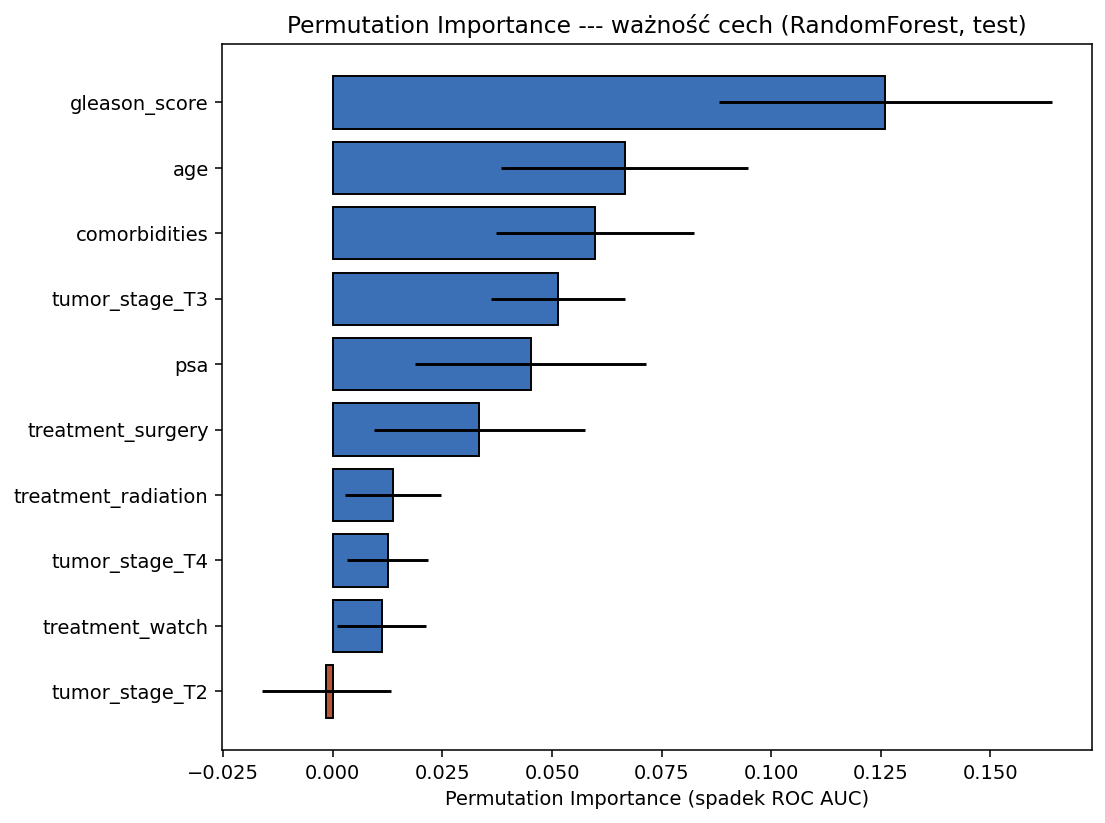
\includegraphics[width=0.85\linewidth]{pi.png}
\caption{Permutation Importance.}
\label{fig:pi}
\end{figure}
\begin{figure}[H]
\centering
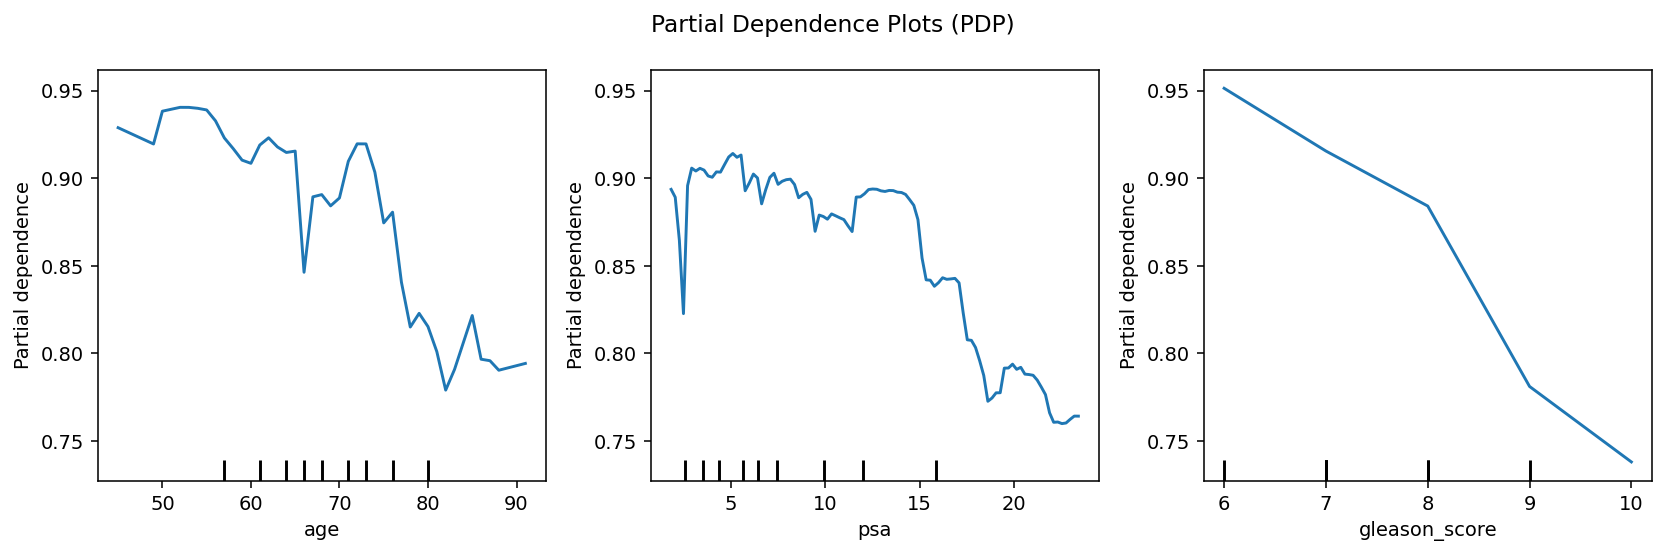
\includegraphics[width=0.85\linewidth]{pdp.png}
\caption{PDP --- średni wpływ cech.}
\label{fig:pdp}
\end{figure}
\begin{figure}[H]
\centering
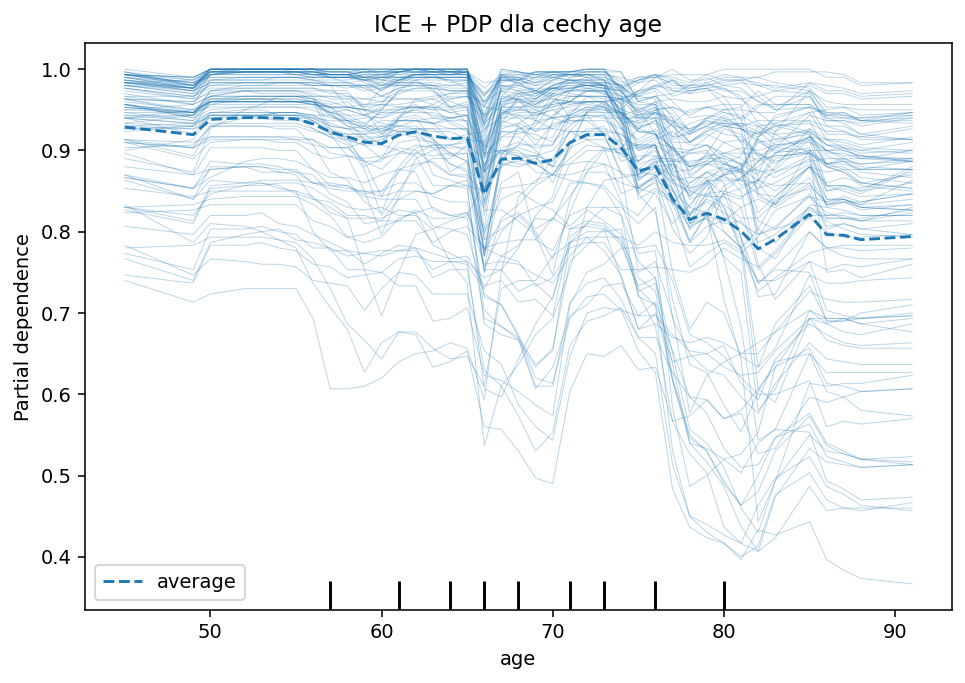
\includegraphics[width=0.85\linewidth]{ice_age.png}
\caption{ICE + PDP dla cechy \texttt{age}.}
\label{fig:ice-age}
\end{figure}
\begin{figure}[H]
\centering
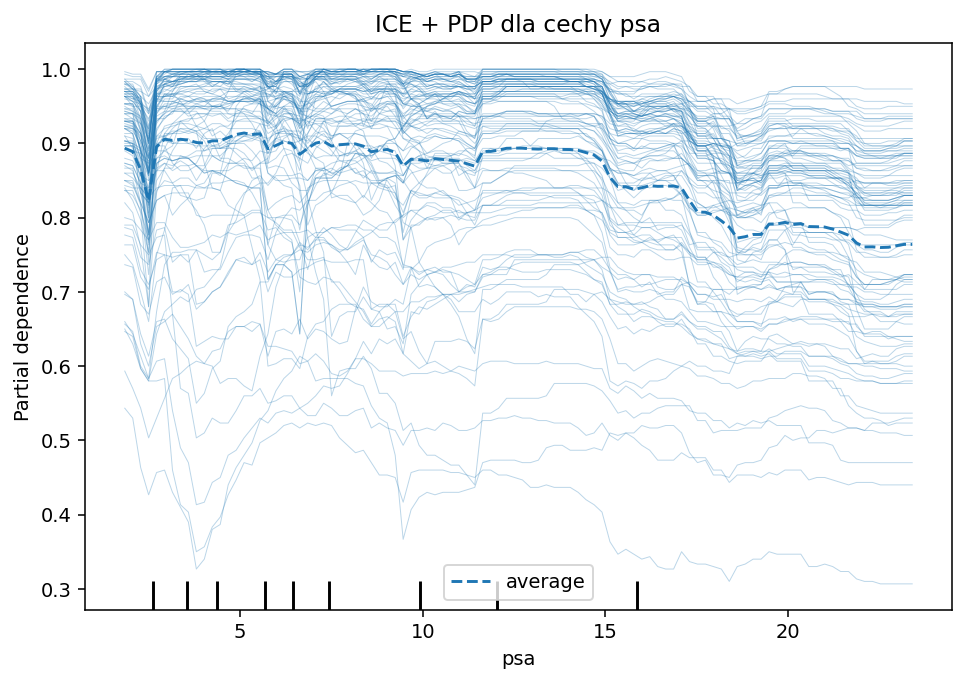
\includegraphics[width=0.85\linewidth]{ice_psa.png}
\caption{ICE + PDP dla cechy \texttt{psa}.}
\label{fig:ice-psa}
\end{figure}
\begin{figure}[H]
\centering
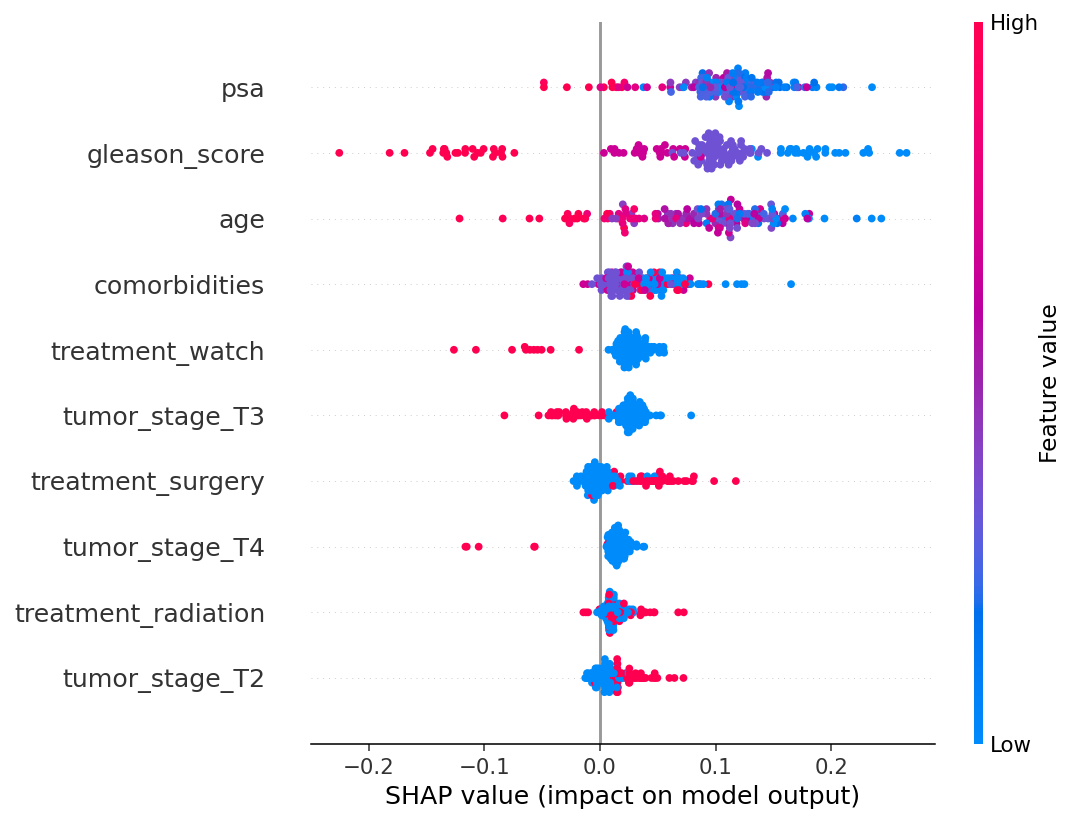
\includegraphics[width=0.85\linewidth]{shap_summary.png}
\caption{SHAP summary plot (TreeExplainer).}
\label{fig:shap-sum}
\end{figure}
\begin{figure}[H]
\centering
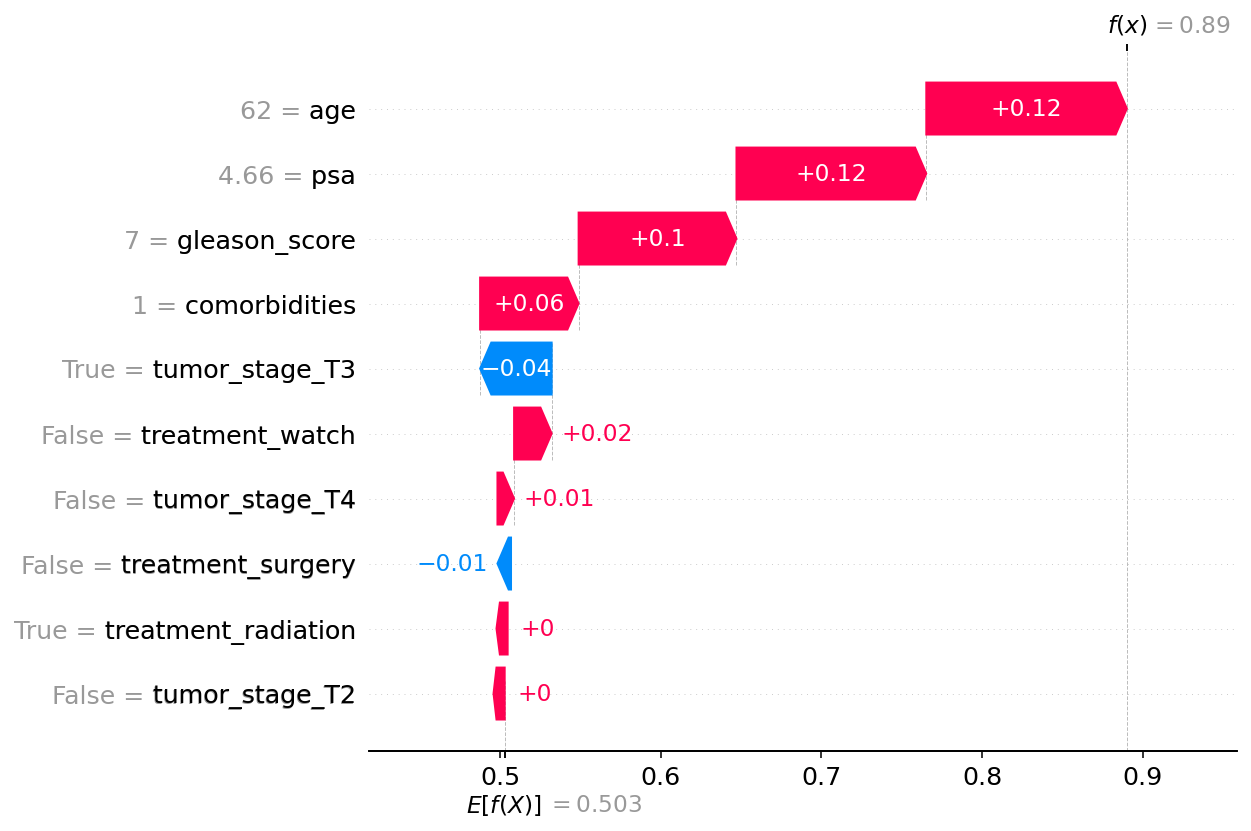
\includegraphics[width=0.85\linewidth]{shap_waterfall_0.png}
\caption{SHAP waterfall --- pacjent \#0.}
\label{fig:shap-wf}
\end{figure}
\begin{figure}[H]
\centering
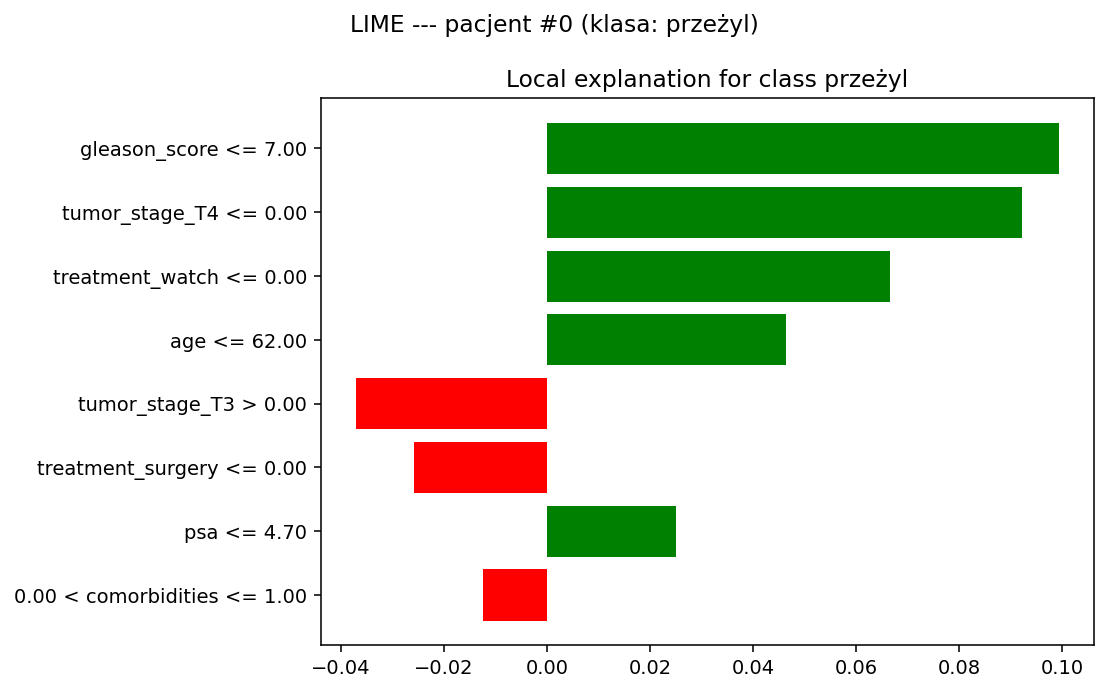
\includegraphics[width=0.85\linewidth]{lime_0.png}
\caption{LIME --- wyjaśnienie pacjenta \#0.}
\label{fig:lime-fig}
\end{figure}


\section{Interpretacja wyników}
PDP \texttt{psa} pokazuje rosnący trend prawdopodobieństwa zgonu wraz ze wzrostem PSA, zgodny z wiedzą kliniczną. ICE \texttt{age} ujawnia heterogeniczność: dla pacjentów z wysokim Gleason score wpływ wieku jest silniejszy. SHAP summary plot potwierdza ranking PI i dodatkowo pokazuje kierunek wpływu (wysokie PSA $\rightarrow$ większe ryzyko). Waterfall dla pacjenta \#0 wskazuje konkretne cechy, które przesunęły jego predykcję powyżej/poniżej wartości oczekiwanej. LIME daje zgodne, choć bardziej zgrubne, wyjaśnienie (dyskretyzacja cech).

\section{Wnioski}
Komplementarność metod: globalne (PI, SHAP summary) wskazują, na których cechach model polega \textit{statystycznie}, lokalne (SHAP waterfall, LIME) wyjaśniają konkretne decyzje. W zastosowaniach klinicznych zaleca się stosować obie warstwy. Pułapki: skorelowane cechy (np. \texttt{psa} $\sim$ \texttt{gleason\_score}) powodują rozdzielanie wpływu, a model może zaniżać PI dla zbędnych zmiennych.

\end{document}
